\documentclass[tikz,border=12pt]{standalone}
% Shared visual language for standalone EMT block diagrams.
\usepackage{amsmath}
\usetikzlibrary{arrows.meta,backgrounds,calc,fit,positioning}

\tikzset{
    emt diagram/.style = {>={Stealth[length=2.4mm]}},
    line/.style        = {semithick, rounded corners=6pt},
    block/.style       = {draw, semithick, fill=white,
                          minimum height=1cm, minimum width=2.3cm},
    hblock/.style      = {block, minimum width=2.24cm, minimum height=1.3cm},
    vblock/.style      = {block, minimum width=1.3cm, minimum height=2.24cm},
    sum/.style         = {draw, semithick, fill=white, circle,
                          inner sep=2.6pt},
    signal/.style      = {circle, fill, inner sep=1.4pt,
                          label distance=3pt},
    sig/.style         = {font=\small},
    pm/.style          = {font=\scriptsize},
    wire jump/.style   = {line,
                          preaction={draw=white, line width=3pt,
                                     line cap=round}},
    enclosure/.style   = {draw, dashed, semithick, rounded corners=4pt},
    operator enclosure/.style = {enclosure, inner xsep=7mm, inner ysep=6mm}
}


% TUNABLES: channel spacing and control-block width.
\def\channelspacing{2.9}
\def\controlwidth{4.4cm}

\begin{document}
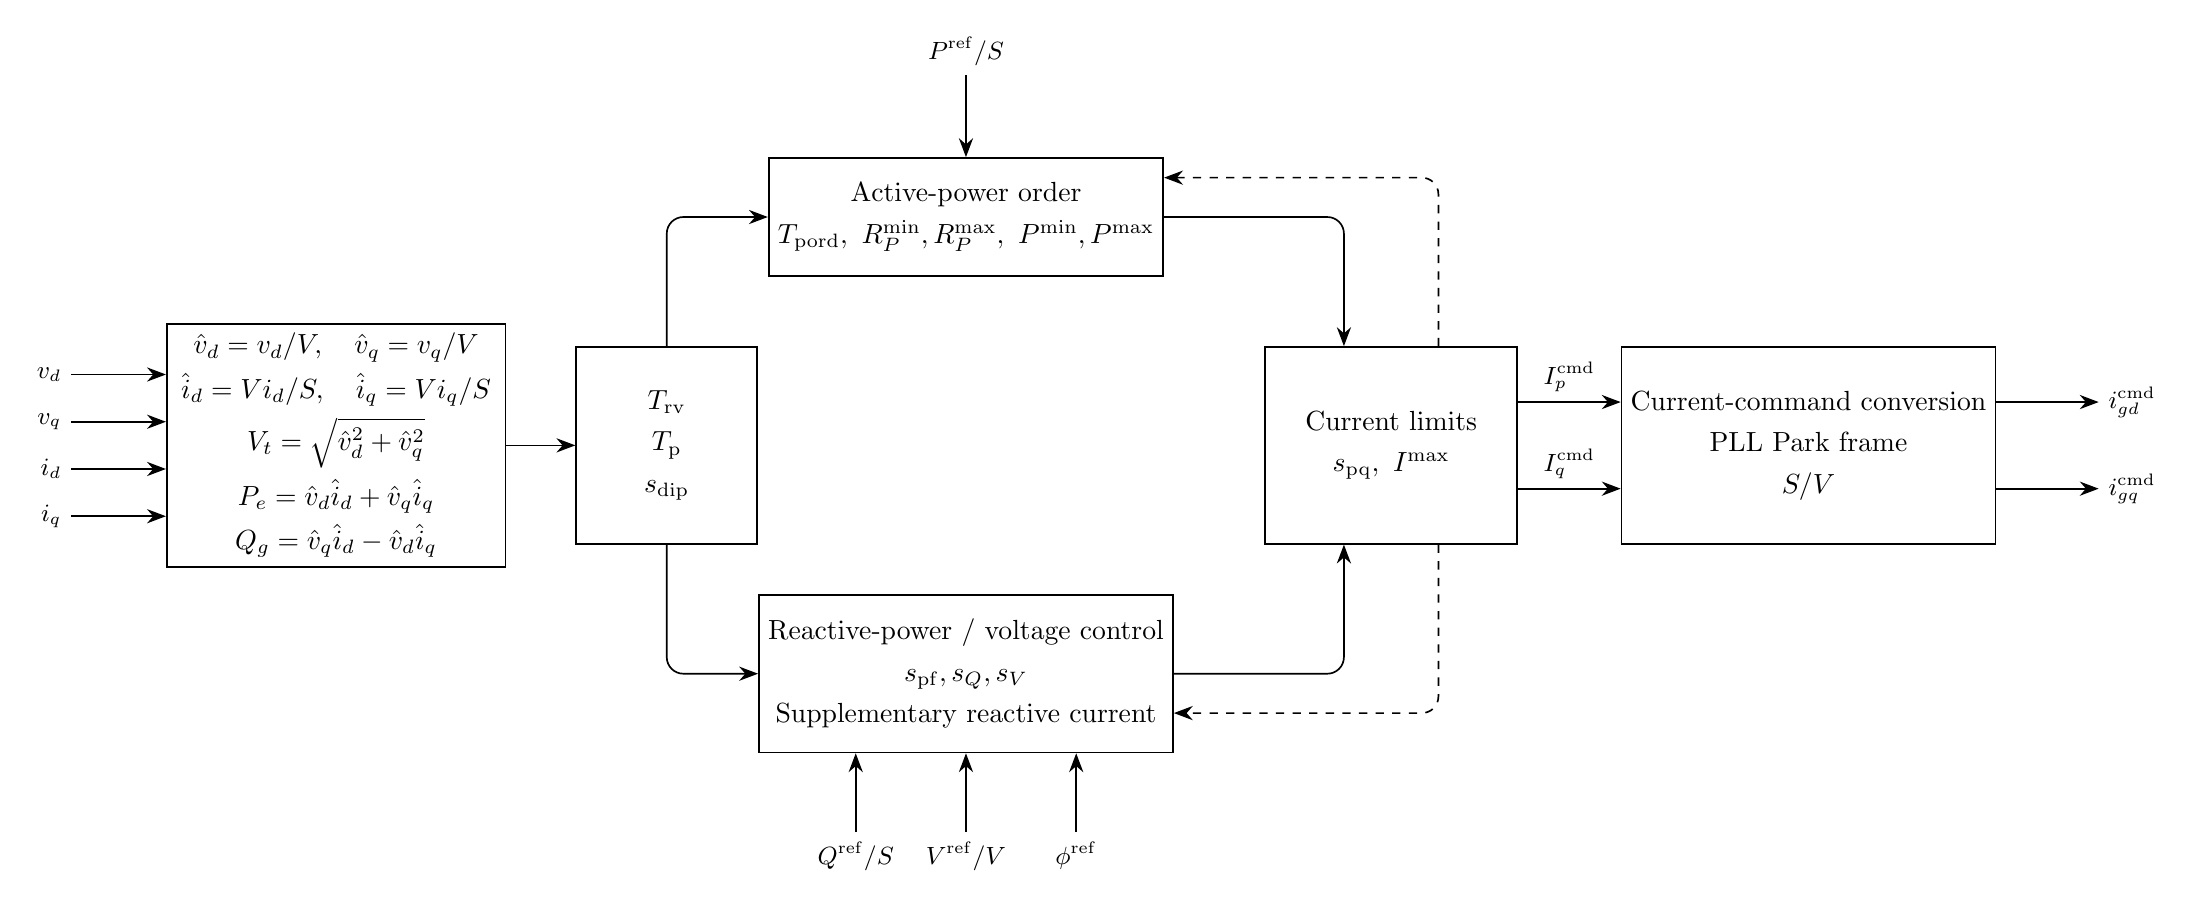
\begin{tikzpicture}[emt diagram,block/.append style={align=center}]
\node[block,minimum width=4.3cm,minimum height=2.8cm] (measure) at (0,0)
    {$\hat v_d=v_d/V,\quad\hat v_q=v_q/V$\\[3pt]
     $\hat i_d=Vi_d/S,\quad\hat i_q=Vi_q/S$\\[3pt]
     $V_t=\sqrt{\hat v_d^2+\hat v_q^2}$\\[3pt]
     $P_e=\hat v_d\hat i_d+\hat v_q\hat i_q$\\[3pt]
     $Q_g=\hat v_q\hat i_d-\hat v_d\hat i_q$};
\foreach \label/\shift in {v_d/0.9,v_q/0.3,i_d/-0.3,i_q/-0.9}
    \draw[->,line] ([xshift=-1.2cm,yshift=\shift cm]measure.west)
        node[sig,left] {$\label$} -- ([yshift=\shift cm]measure.west);

\node[block,minimum width=\controlwidth,minimum height=1.5cm] (active) at (8,\channelspacing)
    {Active-power order\\[3pt]$T_{\mathrm{pord}},\ R_P^{\min},R_P^{\max},\ P^{\min},P^{\max}$};
\draw[->,line] (8,4.7) node[sig,above] {$P^{\mathrm{ref}}/S$} -- (active.north);
\node[block,minimum width=\controlwidth,minimum height=2cm] (reactive) at (8,-\channelspacing)
    {Reactive-power / voltage control\\[3pt]
     $s_{\mathrm{pf}},s_Q,s_V$\\[3pt]
     Supplementary reactive current};
\foreach \label/\shift in {{Q^{\mathrm{ref}}/S}/-1.4,{V^{\mathrm{ref}}/V}/0,\phi^{\mathrm{ref}}/1.4} {
    \draw[->,line] ([yshift=-1cm,xshift=\shift cm]reactive.south)
        node[sig,below] {$\label$} -- ([xshift=\shift cm]reactive.south);
}

\node[block,minimum width=2.3cm,minimum height=2.5cm] (sense) at (4.2,0)
    {$T_{\mathrm{rv}}$\\[3pt]$T_{\mathrm p}$\\[3pt]$s_{\mathrm{dip}}$};
\draw[->,line] (measure.east) -- (sense.west);
\draw[->,line] (sense.north) |- (active.west);
\draw[->,line] (sense.south) |- (reactive.west);

\node[block,minimum width=3.2cm,minimum height=2.5cm] (limit) at (13.4,0)
    {Current limits\\[3pt]$s_{\mathrm{pq}},\ I^{\max}$};
\draw[->,line] (active.east) -| ([xshift=-0.6cm]limit.north);
\draw[->,line] (reactive.east) -| ([xshift=-0.6cm]limit.south);
\draw[->,line,dashed] ([xshift=0.6cm]limit.north) |- ([yshift=0.5cm]active.east);
\draw[->,line,dashed] ([xshift=0.6cm]limit.south) |- ([yshift=-0.5cm]reactive.east);

\node[block,minimum width=3.5cm,minimum height=2.5cm] (project) at (18.7,0)
    {Current-command conversion\\[3pt]PLL Park frame\\[3pt]$S/V$};
\draw[->,line] ([yshift=0.55cm]limit.east) -- node[sig,above] {$I_p^{\mathrm{cmd}}$} ([yshift=0.55cm]project.west);
\draw[->,line] ([yshift=-0.55cm]limit.east) -- node[sig,above] {$I_q^{\mathrm{cmd}}$} ([yshift=-0.55cm]project.west);
\draw[->,line] ([yshift=0.55cm]project.east) -- ++(1.3,0) node[sig,right] {$i_{gd}^{\mathrm{cmd}}$};
\draw[->,line] ([yshift=-0.55cm]project.east) -- ++(1.3,0) node[sig,right] {$i_{gq}^{\mathrm{cmd}}$};
\end{tikzpicture}
\end{document}
